\documentclass{article}
\usepackage[utf8]{inputenc}
\usepackage{xspace}
\usepackage[top=1.5cm, bottom=1.5cm, left=1.5cm, right=1.5cm]{geometry}
\usepackage{enumitem}
\usepackage{graphicx}
\usepackage{textcomp}
\usepackage{amssymb}
\usepackage{ifsym}
\usepackage{xspace}
\usepackage{amsmath}
\usepackage{stmaryrd}
\usepackage{listings}[language=Sql]
\usepackage{xcolor}
\usepackage[labelformat=empty]{caption}

\definecolor{codegreen}{rgb}{0,0.6,0}
\definecolor{codegray}{rgb}{0.5,0.5,0.5}
\definecolor{codepurple}{rgb}{0.58,0,0.82}
\definecolor{backcolour}{rgb}{0.95,0.95,0.92}

\lstdefinestyle{mystyle}{
    language=sql,
    backgroundcolor=\color{backcolour},   
    commentstyle=\color{codegreen},
    keywordstyle=\color{codepurple},
    numberstyle=\tiny\color{codegray},
    stringstyle=\color{codepurple},
    basicstyle=\ttfamily\footnotesize,
    breakatwhitespace=false,         
    breaklines=true,                 
    captionpos=b,                    
    keepspaces=true,                 
    numbers=left,                    
    numbersep=5pt,                  
    showspaces=false,                
    showstringspaces=false,
    showtabs=false,                  
    tabsize=2
}

\lstset{style=mystyle}

\title{Facultad de Ciencias. \\Tarea 6 \\ Fundamentos de Bases de             Datos.}
\author{Arteaga Hernández Alejandro Iabin \and 
        Barocio Gómez Luis Fernando \and 
        Ledesma Granados Roberto Andrés \and
        Castrejón Estrada Juan Carlos}
\date{Entrega 22 de Mayo 2020}

\begin{document}

\maketitle
\begin{enumerate}
    %***************PREGUNTA ! **************************%
    \item Se pide que ajustes el modelo E/R para permitir que un médico pueda ser a su vez paciente. Proporciona el modelo E/R ajustado.
    
    Para lograr que un médico pueda ser ser a la vez paciente, se agrego la relación 
    uno a uno, entre paciente y médico, de esta manera cualquier médico puede tener asociada
    su información como paciente.
    
    \begin{figure}[h]
        \centering
        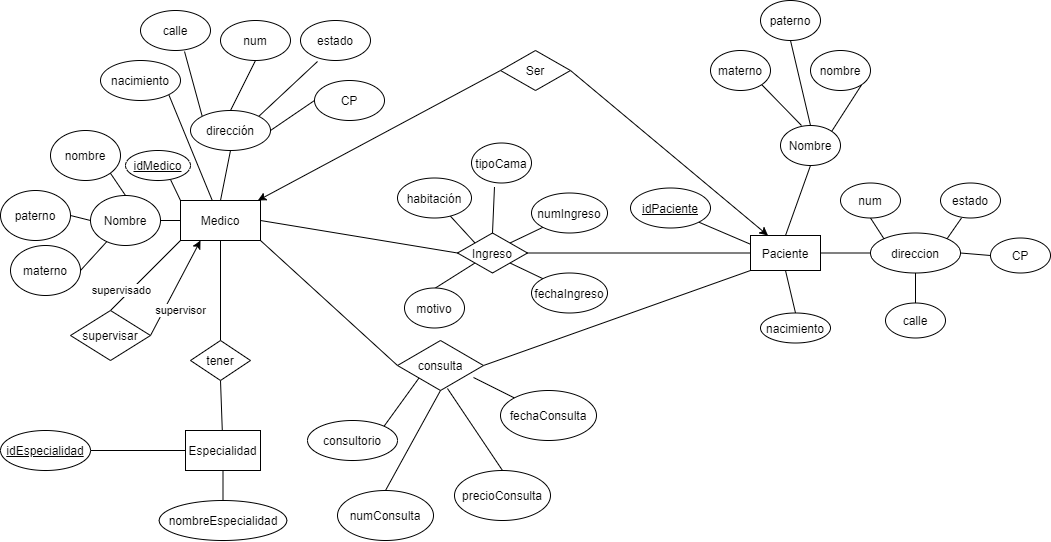
\includegraphics[scale=0.5]{1.png}
        \caption{Diagrama adaptado para que un doctor pueda ser paciente.}
        \label{fig:pregunta1}
    \end{figure}
    
    
    \item Traduce el modelo E/R del punto anterior a su correspondiente modelo relacional, indicando claramente las llaves primarias y foráneas. No incluyas relaciones redundantes.
    
    
    
    Se transformó a modelo relacional, se guarda la información de médicos y pacientes juntos,
    en tablas unidas, debido a que así no hay duplicidad en la información de médicos que sean pacientes, a la tabla persona se le agrega un valor para saber si es un paciente, se agregó el catalogo de especialidades, donde un médico puede ejercer una o varias, las tablas que modelan la lógica de negocio son las consultas y los ingresos, como ambas son relaciones 
    muchos a muchos, se crearon tablas para la información y tablas para contener las relaciones.
    
    Cabe resaltar que este modelo relacional está \textbf{Normalizado} en BCNF ya que para todo
    atributo de toda relación, ese solo depende funcionalmente de la llave primaria.
    
        \begin{figure}[h]
        \centering
        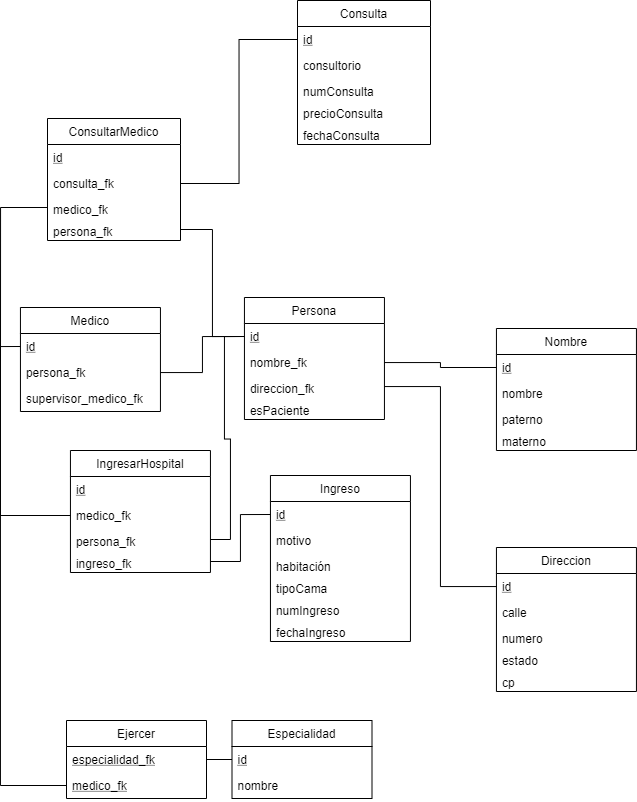
\includegraphics[scale=0.6]{2.png}
        \caption{Modelo relacional}
        \label{fig:pregunta2}
        \end{figure}
    \clearpage
    \item Proporciona un script en SQL que contenga el esquema de cada tabla incluyendo las restricciones de integridad que consideres necesarias. Deberás incluir la totalidad de restricciones que se hayan revisado en clase y/o en laboratorio y debe ser un esquema con integridad referencial. Deberás agregar alguna política de mantenimiento de llaves foráneas.
    
    Pusimos de política que no se puedan borrar elementos con llaves foráneas, ya que lo consideramos mala práctica, trataremos de almacenar la información para que sea siempre accesible, en caso de tener que eliminar datos, estos serán renombrados. por eso ON DELETE NO ACTION
    \begin{lstlisting}
CREATE TABLE consulta(
    id SERIAL PRIMARY KEY,
    consultorio VARCHAR(50),
    numConsulta INTEGER UNIQUE NOT NULL,
    precioConsulta REAL,
    fechaConsulta DATE
);

CREATE TABLE nombre(
    id SERIAL PRIMARY KEY,
    nombre VARCHAR(50),
    paterno VARCHAR(50),
    materno VARCHAR(50)
);

CREATE TABLE direccion(
    id SERIAL PRIMARY KEY,
    calle VARCHAR(50),
    numero VARCHAR(10),
    estado VARCHAR(50),
    cp VARCHAR(5)
);

CREATE TABLE especialidad(
    id SERIAL PRIMARY KEY,
    nombre VARCHAR(50) NOT NULL UNIQUE
);

CREATE TABLE ingreso(
    id SERIAL PRIMARY KEY,
    nombre VARCHAR(50) NOT NULL ,
    paterno VARCHAR(50) NOT NULL ,
    materno VARCHAR(50)
);

CREATE TABLE persona(
    id SERIAL PRIMARY KEY,
    nombre_fk BIGINT REFERENCES nombre(id) ON DELETE NO ACTION,
    direccion_fk BIGINT REFERENCES direccion(id),
    es_paciente BOOLEAN
);

CREATE TABLE medico(
    id SERIAL PRIMARY KEY,
    persona_fk BIGINT REFERENCES persona(id) ON DELETE NO ACTION NOT NULL UNIQUE,
    supervisor_medico_fk BIGINT REFERENCES medico(id)  ON DELETE NO ACTION
);

CREATE TABLE consultar_medico(
    id SERIAL PRIMARY KEY,
    consulta_fk BIGINT REFERENCES consulta(id) ON DELETE NO ACTION,
    medico_fk BIGINT REFERENCES medico(id) ON DELETE NO ACTION,
    persona_fk BIGINT REFERENCES persona(id) ON DELETE NO ACTION
);


CREATE TABLE ingresar_hospital(
    id SERIAL PRIMARY KEY,
    ingreso_fk BIGINT REFERENCES ingreso(id) ON DELETE NO ACTION,
    medico_fk BIGINT REFERENCES medico(id) ON DELETE NO ACTION,
    persona_fk BIGINT REFERENCES persona(id) ON DELETE NO ACTION
);


CREATE TABLE ejercer(
    id SERIAL PRIMARY KEY,
    especialidad_fk BIGINT REFERENCES especialidad(id)  ON DELETE NO ACTION NOT NULL ,
    medico_fk BIGINT REFERENCES medico(id)  ON DELETE NO ACTION NOT NULL
);



\end{lstlisting}

\item[6.] En el caso de la política de mantenimiento de llaves foráneas, indica las ventajas y desventajas que tienen las políticas de establecimiento de nulos y cascada.
\\
Para los nulos:\\
- Ventajas:
\begin{itemize}
    \item Se pueden establecer columnas para datos que por el momento no se tienen o que puedan cambiar de tipo en el futuro
\end{itemize}

- Desventajas:
\begin{itemize}
    \item Hay un riesgo potencial de bugs por el comportamiento de los nulos en los operadores.
    \item Puede haber inconsistencia en la semántica del SQL, cuando se involucran agrupamientos y ordenamientos.
\end{itemize}
Para la cascada:
\\
Ventajas:
\begin{itemize}
    \item Cuando se elimina una fila de la tabla padre, todas las llaves foráneas también son eliminadas
    \item Se evitan filas huérfanas.
\end{itemize}

Desventajas:
\begin{itemize}
    \item Aunque se reduce la posibilidad, puede haber huérfanos
    \item Si por error se elimina una fila en la tabla padre, todas las filas en los hijos serán eliminadas y se toma mucho tiempo en averiguar lo que fue eliminado.
\end{itemize}


    
\end{enumerate}

\end{document}
